\chapter{Introduction}

\section{Background}

% CT studies are pervasive
Computed Tomography (CT) volumetric images have become pervasive in routine clinical practice over the past several decades, numbering in the hundreds of millions per year worldwide, and growing at a fast pace. 
In the USA alone, it is estimated that 10\% of the population has had a CT scan, that the number of scans is 5-10 times higher than in other developed countries, and that about 7 million CT scans are of children.
Radiologists and physicians rely on these images for diagnosis, treatment planning and execution, and follow-up evaluation of a wide range of medical conditions.

% How CT is acquired
During CT acquisition, a gantry consisting of an x-ray tube and an array of detectors is rotated around the patient so that multiple projectional radiography images are collected from many angles (see Fig. \ref{fig:figures/CT_machine.png}).
An algorithm reconstructs a volumetric image from these two dimensional images, wherein each voxel is assigned a value measured in Hounsfield Units (HU) which is closely linked to the linear attenuation coefficient, a physical quantity measuring the absorption of x-rays in the tissue.
The different characteristics of radiation absorption between different types of tissue, along with the ability to inject a contrast agent into the bloodstream, allow CT scans to offer a fast and cost effective method of producing high contrast images of anatomical structures (see Fig. \ref{fig:figures/Brain_CT.png}) while eliminating overlapping structures that are outside the region of interest, giving it clear advantages over traditional 2D radiography.
For these reasons it has become widely used in diagnosis of conditions such as severe trauma, tumors in the abdomen and pelvis, and vascular diseases; in guidance of interventional procedures such as biopsies, aspirations and minimally invasive tumor treatment; and in follow-up assessment of surgical, chemotherapy or other treatments by comparison to pre-treatment scans.

\begin{figure*}[t]
    \centering
    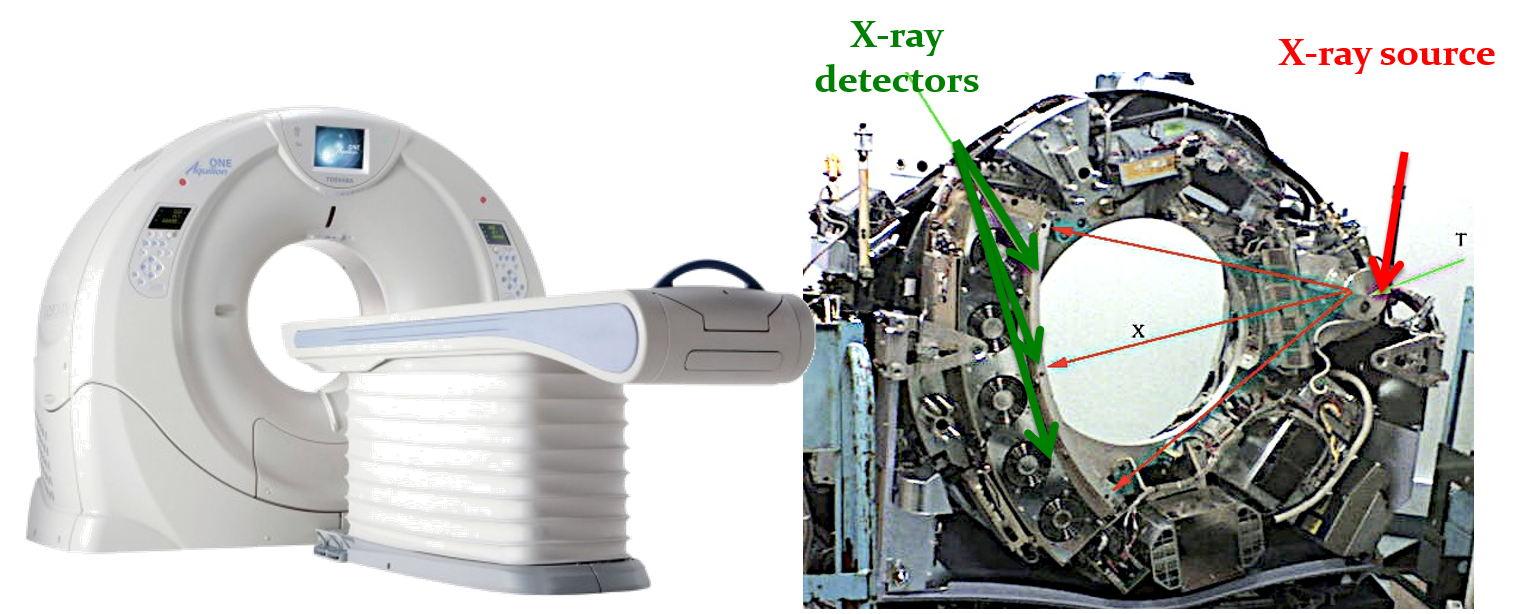
\includegraphics[width=15cm]{figures/CT_machine.png}
    \caption{\small{Left: Computed Tomography (CT) scanner. Right: CT scanner with front cover removed, exposing the x-ray source and detector array on a rotating gantry}}
    \label{fig:figures/CT_machine.png}
\end{figure*}

% harmful radiation
The main disadvantage of CT imaging is that it exposes the patient to a substantial amount of ionizing radiation from x-rays. The radiation dose of a CT scan is the total energy of the x-rays cast onto the patient with sufficient energy to penetrate the structures of the body. The absorbed dose is the energy imparted by ionizing radiation per unit mass of irradiated material. The dose equivalent radiation is a surrogate measure that estimates the hazard to body tissues caused by radiation \cite{mettler2000ct, goo2017dual}. It is cumulative and is quantified in Sievert (Sv) and rem units.
It is now believed that ionizing radiation above a certain threshold may be harmful to the patient \cite{hall2008cancer, davies2011risks, kalra2004strategies}. Studies show that radiation is related to carcinogenesis, which occurs at low doses (\textless 100 mSv) in diagnostic imaging and accounts for an estimated 0.5--0.9\% of cancers. CT-based exams contribute disproportionately to the collective radiation dose of the population. Today, 11\% of diagnostic radiological procedures in the USA are CT examinations. However, their contribution to the collective dose from diagnostic radiology is estimated at 67\% \cite{mettler2000ct}.

The reduction of radiation dose of individual CT scans has become a central clinical and technical issue. In CT imaging, the basic trade-off is between radiation dose and image quality. Lower doses, achieved by fewer X-rays with lower energies, produce imaging artifacts and increased noise, thereby reducing the image quality and limiting its clinical usefulness. Consequently, the clinical indication for CT scan dose determination is the FDA-approved ALARA \textbf{--} As Low As Reasonably Achievable \cite{newman2011alara}. In parallel, many scanning protocols, image reconstruction methods, and clinical evaluation studies have been developed and performed for dose reduction of individual CT scans \cite{shtok2013learned, moore2009adaptive}.

\begin{figure*}[t]
    \centering
    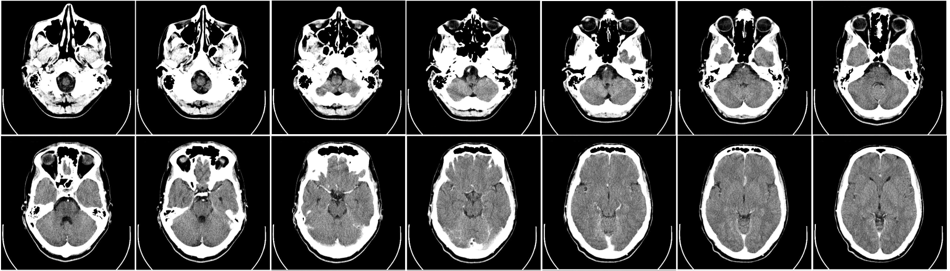
\includegraphics[width=15cm]{figures/Brain_CT.png}
    \caption{\small{Axial slices from a CT scan of the brain.}}
    \label{fig:figures/Brain_CT.png}
\end{figure*}

Repeat CT scanning, in which a patient is scanned some time after a baseline scan was acquired, is very common in many clinical situations, including: 1) multi-phase scanning, in which repeated scanning is performed before and after contrast agent injection \cite{kondo2007mdct}; 2) follow-up scanning, in which repeated scanning is performed for disease progression evaluation, e.g., oncology \cite{zhao2009evaluating}; 3) intra-procedural scanning, in which repeated scanning is performed during an intervention to determine anatomical changes and update the location of tools and catheters; 4) post-procedural scanning, in which repeated scanning is performed to evaluate the procedure results vis-à-vis a pre/intra-procedural scan \cite{thomas2010scheduled, hansen2006repeat}; 5) registration scanning, in which repeated scanning is performed at the start and/or at the end of an intervention to align the pre-procedural scan with the patient; 6) ECG-gated heart scanning, in which repeated scanning is performed to compensate for heart motion \cite{desjardins2004ecg, dafni2013methods}. All repeat scan procedures incur in accumulated radiation, which exacerbates the need for radiation reduction.

This thesis aims to take advantage of the significant, untapped opportunities for dose reduction in repeat CT scanning by incorporating data from the baseline scan in the acquisition and analysis of the repeat scan. The potential is shown, for example, in multi-phase and follow-up studies, where reports indicate that many patients that undergo abdominal and pelvic CT scanning have more that one scan on the same day; that 30\% of them have at least three scans in the course of their treatment \cite{davies2011risks}; and that many receive substantial excess radiation dose with no clinical benefit \cite{mettler2000ct}. Dose reduction is of particular importance in pediatric radiology \cite{donnelly2005reducing, chodick2007excess}.

% fractional scanning
The mechanism by which dose reduction is to be achieved is termed \textit{fractional scanning} in this thesis. 
It is based on the proposition of sparse sampling of the projections in the view-angle domain, i.e. acquiring only a small fraction of the view angles typically acquired in a regular scan.
This scheme would enable reducing the absorbed radiation dose by modulating the x-ray source during gantry rotation, either via current/voltage modulation or fast mechanical collimation.
Fractional scanning is realized in existing CT scanners by tube potential switching and tube current modulation \cite{kalra2004techniques}, and active collimation has been used in radiotherapy \cite{mackie2006history}.
Such alterations to CT scanning firmware and/or hardware are necessary in order to realize the potential of dose reduction using methods presented in this thesis; however, the topic of CT scanner design and control is beyond the scope of this work, which focuses on the algorithmic aspects of leveraging sparse repeat scan data to achieve dose-reduced clinical applications.

\section{Previous work}

Medical image registration has been studied extensively, with several approaches emerging \cite{maintz1998survey}.
\textbf{Feature-based} methods compute the rigid transformation by matching points defined in volumetric medical images, usually of fiducials or natural features, and minimizing the sum of their pairwise distances. Since these methods require the explicit identification and matching of points, their scope is limited to selected clinical scenarios. 
\textbf{Intensity-based} methods perform the registration by comparing the intensity values of both images, a technique which has become dominant in image registration over the past decades \cite{viergever2016survey}. To yield adequate results, they require both volumetric images to be of good quality, be free of image reconstruction artifacts, and have small scanned subject/pose discrepancies.

Specific to the domain of medical images based on radiography (x-ray and CT imaging), \textbf{intensity-based 2D x-ray to 3D CT} registration methods have been developed. Some are in routine clinical use for image-guided therapy and for patient positioning during treatment (see \cite{markelj2012review} for a comprehensive survey). In all cases, the matching procedure requires at least two (and often more) x-ray images of sufficient quality for the matching. The drawbacks of these methods are that they may use different hardware for CT and x-ray acquisition, and that they require set-up time.

\textbf{Radon-space methods}, also called sinogram or projection-space methods, use the CT scans Radon transform representation (sinograms) for the registration. They are not subject to image reconstruction artifacts and have the potential to yield robust and accurate results with greatly reduced doses.
Freiman et al. \cite{freiman2011spectral} describe a 2D/3D registration method for x-ray to CT scans that uses invariant Fourier space features to find the transformation parameters by out-of-plane coarse registration followed by in-plane fine registration. 
Mao et al. \cite{mao2007ct} describe a slice-by-slice registration method in 2D Radon space and its extension to 3D for small angles.
Mooser et al. \cite{mooser2013estimation} propose an iterative optimization method to compute the registration parameters in 3D Radon space for full scans. 
You et al. \cite{you1998image} investigate the invariant properties of rigid movement in image and Radon space. 
Based on this work, Lu, Fitchard et al. \cite{lu1999image, fitchard1998registration, fitchard1999six} use Fourier phase matching to iteratively compute the rigid registration parameters by decomposing the 3D problem into a series of 2D in-plane registrations. The method is limited to small transformations. 

More recently, Wein et al. \cite{wein2011detecting}, Aichert et al. \cite{aichert2014redundancies,aichert2015epipolar}, and Debbler et al \cite{debbeler2013new} use directed epipolar geometry to establish consistency metrics between different projection views for the detection of mid-scan patient motion. However, inter-scan registration is not addressed. 
The 2D Radon transform was shown to be very useful for pattern matching and registration of 2D images, both in terms of accuracy, convergence range and noise robustness \cite{nacereddine2015similarity, wan2010fast}. However, the authors do not indicate how their methods can be extended to 3D and to real sinogram data. 

Deformable registration methods in projection space are also addressed. 
Osorio et al. \cite{osorio2007non} describe a Fourier space based on full CT scans.
Zhang et al. \cite{zhang2014few} present a method that iteratively matches the repeat scan projection to the re-projected deformed baseline. The method requires a preceding rigid registration step to allow convergence of the deformation field to the optimal solution.  
Large reductions in radiation dose have been shown for 3D/2D registration between CT and C-arm fluoroscopy \cite{uneri2014evaluation}.

Chapters \ref{chapters/Reduced-dose_imageless_needle.pdf}-\ref{chapters/Flexible_needle.pdf} focus on clinical applications built on the ability to register a sparse repeat scan to a baseline, namely -- rigid and flexible needle localization. Localization of surgical instruments in CT imaging, and needles in particular, has been addressed in a variety of ways. The needle is usually localized in image space, and so is often required to be inserted in the axial imaging plane (in-plane insertion), which forces the radiologist to adjust the gantry angle repeatedly and re-scan until a suitable orientation is found \cite{walsh2011smaller}. Steering the needle inside the tissue toward the target can be achieved manually by the radiologist under passive guidance, or by robotic steering in closed loop with the imaging. A commercial CT navigation device, SimpliCT by NeoRad \cite{simpliCT}, implements laser steering to guide the radiologist during manual insertion by aligning the needle with the laser direction. In \cite{schubert2013ct}, an optical tracking system uses surface markers to allow feedback of the needle orientation during the intervention. Another approach is to optically over-lay the CT image on top of the patient using a semi-transparent mirror, thereby providing the physician with visual guidance during manual needle insertion \cite{fichtinger2005image}.

Several works describe specific methods to localize the needle shape in reconstructed CT images, relying on acquisition of full repeat scan and reconstruction of the image for each localization of the needle.
Hou et al. \cite{huo2015shape} reconstruct the bevel-tip flexible needle trajectory from full CT slices by localizing points at which the needle intersects slice planes, and fitting a four-order polynomial to the collection of 3D points.
Yaniv et al. \cite{yaniv2010needle} describe a system in which embedded electromagnetic fiducials are used for needle tracking under CT guidance, with operator input required to identify the needle tip in a full CT scan taken in-situ.

The needle shape can be used for control loop feedback in image guided actuated intervention systems.
Ben-David et al. \cite{ben2018evaluation} describe a robotic system for flexible needle insertion under CT guidance. A dual guiding mechanism is composed of a driver which advances the needle while a positioning unit steers it during insertion. A pre-planned 3D trajectory is executed and amended during the insertion based on full repeated CT scans. Earlier work by Glozman et al. \cite{glozman2007image} describes robotic flexible needle steering and a needle-tissue mechanical interaction model, where feedback is based on 2D in-plane imaging of the needle.

\section{Research goals}

\textbf{The first goal of this thesis is to develop and validate an algorithm for rigid registration in repeat CT scanning procedures based on Radon-space methods achieving an x-ray dose reduction.}

The focus of this thesis is to develop methods taking advantage of the information in the baseline scans to reduce the radiation dose required in the follow-up scan. Rigid registration is a cornerstone of computational radiology, and in the case of repeat CT scanning, is an essential preliminary stage in incorporating the information from the baseline and repeat scans in order to produce any clinical value.

\textbf{The second goal is to develop and validate clinical applications leveraging the above registration algorithm, namely: image-less needle tracking methods to allow patient tracking and needle localization intra-operatively.}

The needle tracking solution for interventional radiology realizes the potential of Radon-space rigid registration for dose reduction in a clinical context.

\section{Thesis overview and novelty}

This thesis presents a novel rigid registration method for repeat CT scanning, and a novel application enabled by it in CT guided interventions.

\textbf{The Radon-space rigid registration method} calculates the 6 degrees-of-freedom rigid registration between a baseline scan and a repeat scan without repeat scan image reconstruction and using fractional scanning, which reduces the x-ray dose to which the patient is exposed during the repeat scan.
It is presented in two parts: the first is a method overview for parallel rays geometry with preliminary results using simulated sinogram data obtained from reconstructed CT images. The second part is a theoretical extension to fan- and cone-beam geometries, along with an extensive validation study on parallel rays sinogram data obtained in collaboration with a CT manufacturer - GE Healthcare Haifa.
 
The main advantages of this method are: 
1) out-performs image space registration under sparse sampling conditions;
2) supports much larger transformations than image space registration; 
3) allows for a theoretical dose reduction beyond $\times$100 by combining low tube current scanning and fractional scanning.

\textbf{The rigid needle localization method} builds upon the rigid registration method.
It relies on a spherical marker attached to the needle at a known distance from the tip. The marker is detected in projection difference images, which are generated using the rigid registration obtained using the previous method, and localized in 3D space. Then, the rigid needle direction in 3D space is computed as an intersection of planes associated with the needle projections in the projection difference images.

The main advantages of this method are: 1) it enables existing clinical procedures in interventional radiology to benefit from the potential of x-ray dose reduction; and 2) it accurately localizes the needle with respect to an artifact free baseline scan, without reconstructing the repeat scan image prone to metallic artifacts due to the needle.

\textbf{The flexible needle localization method} extends the rigid needle localization method to expand the range of applicable procedures to those requiring a flexible needle, such as obtaining biopsies of deeply situated targets where sensitive tissue structures must be avoided.
It divides the needle trajectory into short segments and incrementally traces control points along it to generate a curve in 3D space following the needle path.

The main advantage of this method is expanding the applicable procedures of needle based CT-guided interventions to those requiring flexible needles.


\section{Thesis organization}

The rest of this thesis consists of four articles describing the methods listed in the previous section, a discussion, and a list of references. It is organized as follows: 

\textbf{Chapter \ref{chapters/c127-2014-miccai-radon-registration.pdf}}: Reduced-dose patient to baseline CT rigid registration in 3D Radon space.
G. Medan, A. Kronman, L. Joskowicz. International Conference on Medical Image Computing and Computer-Assisted Intervention, p 291-298, 2014.

\textbf{Chapter \ref{chapters/Sparse_3D_Radon_Space_Rigid_Registration.pdf}}: Sparse 3D Radon Space Rigid Registration of CT Scans: Method and Validation Study.
G. Medan, N. Shamul, L. Joskowicz. IEEE Trans. Med. Imaging 36, no. 2 (2017): 497-506.

\textbf{Chapter \ref{chapters/Reduced-dose_imageless_needle.pdf}}: Reduced-Dose Imageless Needle and Patient Tracking in Interventional CT Procedures.
G. Medan, L. Joskowicz. IEEE Trans. Med. Imaging 36, no. 12 (2017): 2449-2456.

\textbf{Chapter \ref{chapters/Flexible_needle.pdf}}: Flexible needle and patient tracking using fractional scanning for reduced dose in interventional CT procedures. Guy Medan and Leo Joskowicz (submitted to IEEE Trans. Med. Imaging). %TODO

\textbf{Chapter \ref{ch:conclusions}}: Discussion and Conclusions

\textbf{References}